
\documentclass[a4paper,10pt]{article}
\usepackage[top=2cm, left=2.5cm, right=2.5cm, bottom=2cm]{geometry}
\usepackage[cmex10]{amsmath}
\usepackage{graphicx}
\usepackage{gvv-book}
\usepackage{gvv}
\usepackage{textcomp}
\usepackage{multicol}

\begin{document}

\title{2009 - AR : Architecture and Planning Exam}
\author{Puni Aditya - EE25BTECH11046}
\date{3rd August, 2025}
\maketitle
Duration: Three Hours \hfill Maximum Marks:100

\section*{Q.1 - Q.20 carry one mark each.}

\begin{enumerate}
    \item The essential difference between CPM and PERT is 
    \begin{enumerate}
        \item Critical Path vs. Critical Activity
        \item Arrow notation vs. Precedence notation
        \item Deterministic approach vs. Probabilistic approach
        \item Project Management vs. Network Analysis
    \end{enumerate}
    \hfill (GATE-AR 2009)
    
    \item The minimum thickness of a wall where single Flemish bond can be used is 
    \begin{enumerate}
        \item Half-brick thick
        \item One-brick thick
        \item One-and-half-brick thick
        \item Two-brick thick
    \end{enumerate}
    \hfill (GATE-AR 2009)
    
    \item On the colour wheel, the combination of 'Violet-Yellow' or 'Orange-Blue' are best described as 
    \begin{multicols}{4}
	\begin{enumerate}
        \item Complementary
        \item Supplementary
        \item Analogous
        \item Monochromatic
    \end{enumerate}
	\end{multicols}
    \hfill (GATE-AR 2009)
    
    \item The sudden stoppage in the flow of water in a closed conduit results in a phenomenon called 
    \begin{multicols}{2}
	\begin{enumerate}
        \item Cavitation
        \item Hydraulic gradient
        \item Stack pressure
        \item Water hammer
    \end{enumerate}
	\end{multicols}
    \hfill (GATE-AR 2009)

    \item The number of intersecting arches that support Bijapur’s Gol Gumbaz is 
    \begin{multicols}{4}
	\begin{enumerate}
        \item 4
        \item 8
        \item 12
        \item 16
    \end{enumerate}
	\end{multicols}
    \hfill (GATE-AR 2009)
    
    \item The 73\textsuperscript{rd} and 74\textsuperscript{th} Constitutional Amendments pertain to 
    \begin{enumerate}
        \item Abolishing the Urban Land Ceiling Act
        \item Providing restricted role to local courts to settle rural disputes
        \item Providing more responsibility to municipal and local bodies for planning and development
        \item Providing right to information for the general public
    \end{enumerate}
    \hfill (GATE-AR 2009)
    
    \item A simply supported beam of length L carries a concentrated load of intensity P at its centre. The bending moment at the centre of the beam will be 
    \begin{multicols}{4}
	\begin{enumerate}
        \item PL/2
        \item PL/4
        \item PL/6
        \item PL/8
    \end{enumerate}
	\end{multicols}
    \hfill (GATE-AR 2009)

    \item 'Desire lines' are associated with 
    \begin{enumerate}
        \item Origin – Destination analysis in transportation planning
        \item Income – Expenditure analysis in personal finance management
        \item Cut – Fill analysis in landscape planning
        \item Demand – Supply analysis in economic planning
    \end{enumerate}
    \hfill (GATE-AR 2009)

	\item GRiHA is a rating for Green Buildings given by 
    \begin{multicols}{2}
	\begin{enumerate}
        \item The Energy Research Institute
        \item Development Alternatives
        \item Bureau of Energy Efficiency
        \item Ministry of Power
    \end{enumerate}
	\end{multicols}
    \hfill (GATE-AR 2009)
    
    \item A 'cul-de-sac' is a street where 
    \begin{enumerate}
        \item Only two-wheelers are permitted
        \item Through traffic is discouraged
        \item Pedestrians are not permitted
        \item Vehicles are permitted to move in one direction only
    \end{enumerate}
    \hfill (GATE-AR 2009)

    \item 'Usonian' houses were designed by 
    \begin{multicols}{2}
	\begin{enumerate}
        \item Mies van der Rohe
        \item Alvar Aalto
        \item Frank Lloyd Wright
        \item Le Corbusier
    \end{enumerate}
	\end{multicols}
    \hfill (GATE-AR 2009)
    
    \item Increase in the volume of fine aggregate due to the presence of moisture is called 
    \begin{multicols}{4}
	\begin{enumerate}
        \item Bulking
        \item Buckling
        \item Bending
        \item Twisting
    \end{enumerate}
	\end{multicols}
    \hfill (GATE-AR 2009)
    
    \item The Pattern Language theory was propounded by 
    \begin{multicols}{2}
	\begin{enumerate}
        \item Christopher Alexander
        \item Patrick Geddes
        \item John Ruskin
        \item Amos Rapoport
    \end{enumerate}
	\end{multicols}
    \hfill (GATE-AR 2009)
    
    \item As per IS:456-2000, the maximum area of tension reinforcement in a RCC beam shall not exceed x\% of its cross-sectional area, where x is equal to 
    \begin{multicols}{4}
	\begin{enumerate}
        \item 2
        \item 4
        \item 6
        \item 8
    \end{enumerate}
	\end{multicols}
    \hfill (GATE-AR 2009)
    
    \item 'No-cut no-fill' lines are mostly used in 
    \begin{multicols}{2}
	\begin{enumerate}
        \item Land use planning
        \item Interpretation of stereo-vision photographs
        \item Earthwork computation
        \item Interpretation of remotely sensed images
    \end{enumerate}
	\end{multicols}
    \hfill (GATE-AR 2009)
    
    \item The property of concrete measured by the Slump Test is 
    \begin{multicols}{4}
	\begin{enumerate}
        \item Durability
        \item Hardness
        \item Strength
        \item Workability
    \end{enumerate}
	\end{multicols}
    \hfill (GATE-AR 2009)
    
    \item The Remote Sensing satellite that gives the highest spatial resolution is 
    \begin{multicols}{4}
	\begin{enumerate}
        \item IKONOS 2
        \item IRS 1C/1D
        \item Quickbird 2
        \item SPOT 5
    \end{enumerate}
	\end{multicols}
    \hfill (GATE-AR 2009)
    
    \item Development that meets the needs of the present generation without compromising the ability of future generations to meet their own needs is termed by UNDP as 
    \begin{multicols}{2}
	\begin{enumerate}
        \item Comprehensive Development
        \item Equitable Development
        \item Human Development
        \item Sustainable Development
    \end{enumerate}
	\end{multicols}
    \hfill (GATE-AR 2009)

	\item The parameter that does NOT apppear in a Psychrometric Chart is 
    \begin{multicols}{2}
	\begin{enumerate}
        \item Wind speed
        \item Dry bulb temperature
        \item Wet bulb temperature
        \item Relative humidity
    \end{enumerate}
	\end{multicols}
    \hfill (GATE-AR 2009)

	\item Allowable stress in the design of a tension member in a steel truss is a function of 
    \begin{enumerate}
        \item Cross-sectional area of the member
        \item Yield stress of the material
        \item Slenderness ratio of the member
        \item Moment of inertia of the member's cross-section
    \end{enumerate}
    \hfill (GATE-AR 2009)

\section*{Q.21 to Q.60 carry two marks each.}

    \item The parameters for determining Human Development Index are: 
    \begin{itemize}
        \item Educational Attainment
        \item Per capita Gross Agricultural Produce
        \item Life Expectancy
        \item Per capita Gross Domestic Product
        \item Per capita State Domestic Product
    \end{itemize}
    \begin{multicols}{4}
	\begin{enumerate}
        \item P, Q, S
        \item P, Q, S, T
        \item P, R, S
        \item R, S, T
    \end{enumerate}
	\end{multicols}
    \hfill (GATE-AR 2009)
    
    \item Match the individuals in Group I with the works in Group II:  \\
    \begin{tabular}{ l l }
	\textbf{Group I} & \textbf{Group II} \\
	P. Hippodamus & 1. Aqueducts \\
	Q. Vitruvius & 2. Campidoglio \\
	R. Michelangelo & 3. Hagia Sophia \\
	S. Constantine & 4. Agora \\
	& 5. Hanging Gardens \\
	\end{tabular}
	\begin{multicols}{2}
	\begin{enumerate}
        \item P-4, Q-1, R-2, S-3
        \item P-3, Q-1, R-2, S-5
        \item P-4, Q-5, R-1, S-3
        \item P-3, Q-4, R-1, S-2
    \end{enumerate}
	\end{multicols}
    \hfill (GATE-AR 2009)
    
    \item If the height of the facade = h, and the distance of the observer from the building = d, then match the enclosure types in Group I with their corresponding h/d ratio in Group II:  \\
    \begin{tabular}{ l l }
	\textbf{Group I} & \textbf{Group II} \\
	P. Full enclosure & 1. 1 \\
	Q. Threshold of enclosure & 2. 1/2 \\
	R. Minimum of enclosure & 3. 1/3 \\
	S. Loss of enclosure & 4. 1/4 \\
	& 5. 1/5 \\
	\end{tabular}
	\begin{multicols}{2}
	\begin{enumerate}
        \item P-1, Q-2, R-3, S-4
        \item P-4, Q-3, R-2, S-1
        \item P-2, Q-3, R-4, S-1
        \item P-5, Q-1, R-2, S-4
    \end{enumerate}
	\end{multicols}
    \hfill (GATE-AR 2009)

	\item The correct sequence of activities in Solid Waste Management is 
    \begin{enumerate}
        \item Collection $\to$ Transportation $\to$ Treatment $\to$ Segregation
        \item Segregation $\to$ Collection $\to$ Transportation $\to$ Treatment
        \item Collection $\to$ Segregation $\to$ Treatment $\to$ Transportation
        \item Treatment $\to$ Collection $\to$ Transportation $\to$ Segregation
    \end{enumerate}
    \hfill (GATE-AR 2009)
    
    \item The principles of Universal Design include: 
    \begin{itemize}
        \item Flexibility in use
        \item Tolerance for error
        \item Energy efficiency
        \item Low physical effort
    \end{itemize}
    \begin{multicols}{4}
	\begin{enumerate}
        \item P, Q, R
        \item Q, R, S
        \item P, R, S
        \item P, Q, S
    \end{enumerate}
	\end{multicols}
    \hfill (GATE-AR 2009)
    
    \item Match the urban design elements in Group I with their descriptions in Group II:  \\
    \begin{tabular}{ l l }
	\textbf{Group I} & \textbf{Group II} \\
	P. District & 1. Recognizable as having some common identifying character \\
	Q. Landmark & 2. Centre of activity \\
	R. Node & 3. Network of major and minor routes \\
	S. Pathway & 4. Prominent visual feature of the city \\
	\end{tabular}
	\begin{multicols}{2}
	\begin{enumerate}
        \item P-3, Q-4, R-2, S-1
        \item P-1, Q-4, R-2, S-3
        \item P-1, Q-2, R-4, S-3
        \item P-2, Q-4, R-1, S-3
    \end{enumerate}
	\end{multicols}
    \hfill (GATE-AR 2009)

    \item A commercial plot measures 100 m $\times$ 80 m. If the permissible Floor Space Index (FSI) is 3.0, and 50\% of the ground is covered, then the maximum number of floors that can be built is 
    \begin{multicols}{4}
	\begin{enumerate}
        \item 3
        \item 4
        \item 6
        \item 12
    \end{enumerate}
	\end{multicols}
    \hfill (GATE-AR 2009)

    \item Match elements of a Buddhist Stupa in Group I with their traditional names in Group II:  \\
	\begin{tabular}{ l l }
	\textbf{Group I} & \textbf{Group II} \\
	P. Hemispherical Dome & 1. Vedika \\
	Q. Peripheral Railing & 2. Anda \\
	R. Entrance Gateway & 3. Harmika \\
	S. Portion above dome & 4. Nagara \\
	& 5. Chaitya \\
	& 6. Torana \\
	\end{tabular}
	\begin{multicols}{2}
	\begin{enumerate}
        \item P-2, Q-1, R-6, S-3
        \item P-2, Q-6, R-4, S-3
        \item P-3, Q-1, R-5, S-2
        \item P-5, Q-6, R-1, S-2
    \end{enumerate}
	\end{multicols}
    \hfill (GATE-AR 2009)

    \item A microwave oven of 3 kW rating is operated for 30 minutes, a hot water geyser of 1 kW rating is operated for 15 minutes, and 5 fluorescent lamps of 60 W are operated for 6 hours. The total power consumed (in kWh) will be 
    \begin{multicols}{4}
	\begin{enumerate}
        \item 1.80
        \item 3.55
        \item 18.01
        \item 35.50
    \end{enumerate}
	\end{multicols}
    \hfill (GATE-AR 2009)

    \item Match the building projects in Group I with their architects in Group II:  \\
    \begin{tabular}{ l l }
	\textbf{Group I} & \textbf{Group II} \\
	P. National Olympic Stadium, Beijing & 1. Rem Koolhaas \\
	Q. Glass Pyramid, the Louvre, Paris & 2. Richard Rogers \\
	R. Millennium Dome, London & 3. Renzo Piano \\
	S. Kansai Airport, Osaka & 4. Tadao Ando \\
	& 5. I. M. Pei \\
	& 6. Herzog \& de Meuron \\
	\end{tabular}
	\begin{multicols}{2}
	\begin{enumerate}
        \item P-6, Q-2, R-3, S-4
        \item P-1, Q-6, R-2, S-4
        \item P-6, Q-5, R-2, S-3
        \item P-2, Q-5, R-1, S-3
    \end{enumerate}
	\end{multicols}
    \hfill (GATE-AR 2009)

    \item Identify the ‘pre-historic’ structures in the following: 
    \begin{itemize}
        \item Mastaba
        \item Dolmen
        \item Menhir
        \item Pylon
        \item Stonehenge
        \item Thermae
    \end{itemize}
    \begin{multicols}{4}
	\begin{enumerate}
        \item P, Q, R
        \item R, T, U
        \item Q, S, T
        \item Q, R, T
    \end{enumerate}
	\end{multicols}
    \hfill (GATE-AR 2009)

    \item Match the figures of cut bricks in Group I with their terms in Group II:  \\
    \begin{tabular}{ l }
	\textbf{Group I} \\
	\end{tabular}
	\begin{figure}[h!]
        \centering
        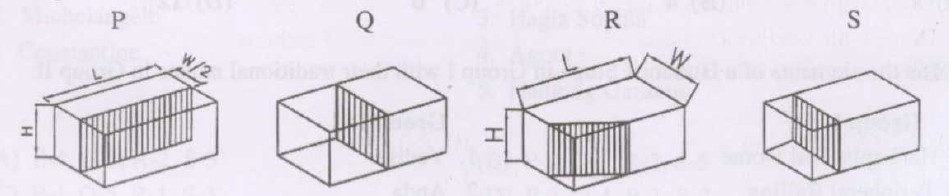
\includegraphics[width=0.5\linewidth]{figs/01.jpg}
        \label{fig:Img01}
	\caption{Figures of Cut Bricks}
	\end{figure}
    \begin{tabular}{ l l l l }
	\textbf{Group II} & & & \\
	1. King Closer & 2. Queen Closer & 3. Half Bat & 4. Three Quarter Bat \\
	\end{tabular}
	\begin{multicols}{2}
	\begin{enumerate}
        \item P-2, Q-3, R-1, S-4
        \item P-2, Q-1, R-3, S-4
        \item P-1, Q-2, R-4, S-3
        \item P-3, Q-4, R-1, S-2
    \end{enumerate}
	\end{multicols}
    \hfill (GATE-AR 2009)

    \item A site has 6 contour lines and the length of the line joining the midpoints of the highest contour and lowest contour is 300 m. If the slope of the line is 1 in 10, then the contour interval (in m) is 
    \begin{multicols}{4}
	\begin{enumerate}
        \item 5
        \item 6
        \item 50
        \item 60
    \end{enumerate}
	\end{multicols}
    \hfill (GATE-AR 2009)
	
	\item Match the plant types in Group I with their corresponding examples in Group II:  \\
    \begin{tabular}{ l l }
	\textbf{Group I} & \textbf{Group II} \\
	P. Climber & 1. Croton \\
	Q. Shrub & 2. Shirish \\
	R. Tree & 3. Duranta \\
	S. Hedge & 4. Bougainvillea \\
	\end{tabular}
	\begin{multicols}{2}
	\begin{enumerate}
        \item P-3, Q-1, R-2, S-4
        \item P-2, Q-4, R-1, S-3
        \item P-4, Q-1, R-2, S-3
        \item P-4, Q-3, R-1, S-2
    \end{enumerate}
	\end{multicols}
    \hfill (GATE-AR 2009)

    \item A neighbourhood with a total area of 200 hectares has a gross density of 300 persons per hectare (pph). If the residential area is 60\% of the total area, then net density (in pph) of the neighbourhood is 
    \begin{multicols}{4}
	\begin{enumerate}
        \item 300
        \item 450
        \item 500
        \item 750
    \end{enumerate}
	\end{multicols}
    \hfill (GATE-AR 2009)

    \item Identify the parameters used in the Hazen \& William’s nomogram to calculate pipe diameter for water supply: 
    \begin{itemize}
        \item Flow rate in lit/sec
        \item Pipe diameter in mm
        \item Population to be served
        \item Head loss in m/m
        \item Velocity in m/sec
    \end{itemize}
    \begin{multicols}{4}
	\begin{enumerate}
        \item P, Q, S
        \item R, S, T
        \item P, R, S
        \item P, S, T
    \end{enumerate}
	\end{multicols}
    \hfill (GATE-AR 2009)

    \item Match the domes in Group I with their examples in Group II:  \\
    \begin{tabular}{ l l }
	\textbf{Group I} & \textbf{Group II} \\
	P. Dome with a huge central cut-out at the top & 1. Pisa Cathedral \\
	Q. Dome with slit windows at the springing level & 2. St. Peter’s Cathedral \\
	R. Dome with an elliptical base & 3. Pantheon \\
	S. Dome on a drum with a lantern on top & 4. Hagia Sophia \\
	\end{tabular}
	\begin{multicols}{2}
	\begin{enumerate}
        \item P-2, Q-1, R-3, S-4
        \item P-3, Q-1, R-2, S-4
        \item P-3, Q-4, R-2, S-1
        \item P-3, Q-4, R-1, S-2
    \end{enumerate}
	\end{multicols}
    \hfill (GATE-AR 2009)

    \item Match the Institutions in Group I with their Architects in Group II:  \\
    \begin{tabular}{ l l }
	\textbf{Group I} & \textbf{Group II} \\
	P. National Dairy Development Board, New Delhi & 1. B. V. Doshi \\
	Q. National Institute of Immunology, New Delhi & 2. Charles Correa \\
	R. Indian Institute of Management, Bangalore & 3. A.P. Kanvinde \\
	S. Jodhpur University, Jodhpur & 4. J.A. Stein \\
	& 5. Raj Rewal \\
	& 6. U.C. Jain \\
	\end{tabular}
	\begin{multicols}{2}
	\begin{enumerate}
        \item P-3, Q-5, R-1, S-6
        \item P-6, Q-3, R-4, S-1
        \item P-3, Q-1, R-4, S-6
        \item P-3, Q-4, R-2, S-6
    \end{enumerate}
	\end{multicols}
    \hfill (GATE-AR 2009)

    \item Identify the urban functions that are included under Social Infrastructure: 
    \begin{itemize}
        \item Schools and colleges
        \item Hospitals and clinics
        \item Roads and footpaths
        \item Parks and plazas
        \item Malls and markets
        \item Community centres
    \end{itemize}
    \begin{multicols}{4}
	\begin{enumerate}
        \item P, Q, S, U
        \item P, Q, S, T
        \item P, R, S, U
        \item Q, S, T, U
    \end{enumerate}
	\end{multicols}
    \hfill (GATE-AR 2009)

    \item Match the tombs in Group I with their architectural characteristics in Group II:  \\
    \begin{tabular}{ l l }
	\textbf{Group I} & \textbf{Group II} \\
	P. Tomb of Sher Shah & 1. Irregular pentagonal site plan \\
	Q. Tomb of Ghias-ud-din Tughlaq & 2. Octagonal plan \\
	R. Humayun’s tomb & 3. Gateway with four minarets \\
	S. Akbar’s tomb & 4. Persian dome \\
	\end{tabular}
	\begin{multicols}{2}
	\begin{enumerate}
        \item P-4, Q-1, R-2, S-3
        \item P-2, Q-1, R-4, S-3
        \item P-4, Q-3, R-2, S-1
        \item P-2, Q-3, R-1, S-4
    \end{enumerate}
	\end{multicols}
    \hfill (GATE-AR 2009)

    \item Match the high-rise tube structural systems in Group I with their corresponding terms in Group II:  \\
    \begin{tabular}{ l }
	\textbf{Group I} \\
	\end{tabular}
	\begin{figure}[h!]
        \centering
        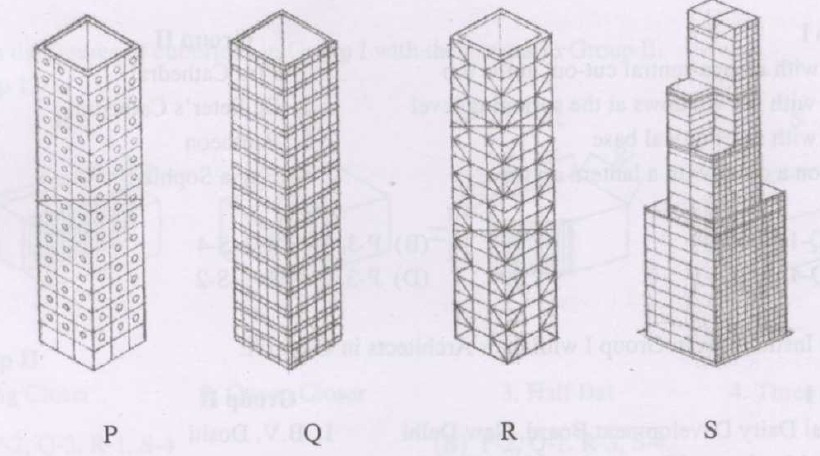
\includegraphics[width=0.5\linewidth]{figs/02.jpg}
	\caption{High-Rise Tube Structural Systems}
    \label{fig:Img02}
	\end{figure}
    \begin{tabular}{ l l l l }
	\textbf{Group II} & & & \\
	1. Framed tube & 2. Bundled tubes & 3. Braced tube & 4. Perforated shell tube \\
	\end{tabular}
	\begin{multicols}{2}
	\begin{enumerate}
        \item P-1, Q-3, R-2, S-4
        \item P-4, Q-1, R-3, S-2
        \item P-4, Q-1, R-2, S-3
        \item P-1, Q-4, R-3, S-2
    \end{enumerate}
	\end{multicols}
    \hfill (GATE-AR 2009)

    \item A town with a population of 50000 has an average household size of 5.0. The number of occupied dwelling units is 8400 of which 10\% are in dilapidated condition. The housing demand of the town is 
    \begin{multicols}{4}
	\begin{enumerate}
        \item 760
        \item 1600
        \item 2440
        \item 10840
    \end{enumerate}
	\end{multicols}
    \hfill (GATE-AR 2009)

    \item Match the items in Group I with those in Group II:  \\
    \begin{tabular}{ l l }
	\textbf{Group I} & \textbf{Group II} \\
	P. Hypostyle hall & 1. Roman architecture \\
	Q. Ziggurat & 2. Egyptian architecture \\
	R. Acropolis & 3. Assyrian architecture \\
	S. Triumphal arch & 4. Greek architecture \\
	\end{tabular}
	\begin{multicols}{2}
	\begin{enumerate}
        \item P-1, Q-3, R-4, S-2
        \item P-2, Q-3, R-1, S-4
        \item P-1, Q-4, R-2, S-3
        \item P-2, Q-3, R-4, S-1
    \end{enumerate}
	\end{multicols}
    \hfill (GATE-AR 2009)

    \item Match the Planning Models in Group I with their proponents in Group II:  \\
    \begin{tabular}{ l }
	\textbf{Group I} \\
	\end{tabular}
	\begin{figure}[h!]
        \centering
        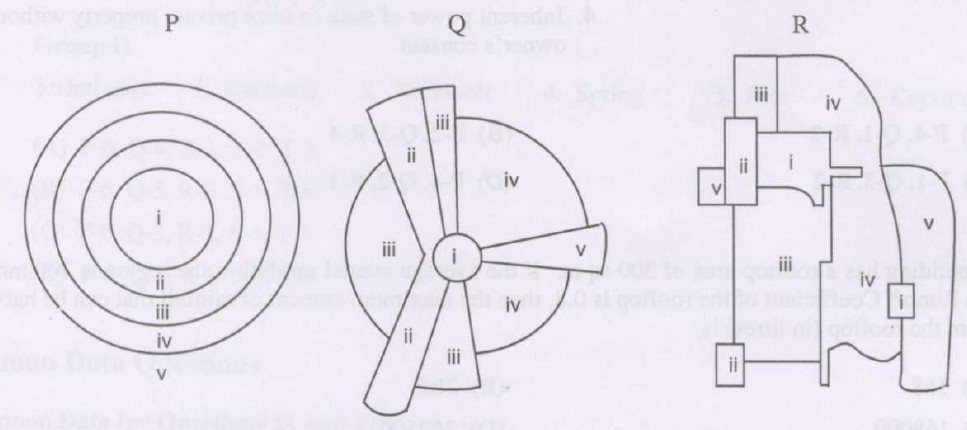
\includegraphics[width=0.5\linewidth]{figs/03.jpg}
	\caption{Planning Models}
	\label{fig:Img03}
	\end{figure}
    \begin{tabular}{ l l l l l }
	\textbf{Group II} & & \\
	1. Homer Hoyt & 2. Ernest Burgess & 3. Von Thunen & 4. Harris \& Ullman & 5. William Reilley \\
	\end{tabular}
	\begin{multicols}{2}
	\begin{enumerate}
        \item P-1, Q-4, R-5
        \item P-2, Q-1, R-4
        \item P-4, Q-1, R-2
        \item P-3, Q-2, R-1
    \end{enumerate}
	\end{multicols}
    \hfill (GATE-AR 2009)

    \item The correct sequence in the four-stage model used for transportation planning is 
    \begin{enumerate}
        \item Trip generation $\to$ Trip distribution $\to$ Modal split $\to$ Trip assignment
        \item Trip generation $\to$ Trip assignment $\to$ Modal split $\to$ Trip distribution
        \item Trip distribution $\to$ Modal split $\to$ Trip assignment $\to$ Trip generation
        \item Trip generation $\to$ Trip distribution $\to$ Trip assignment $\to$ Modal split
    \end{enumerate}
    \hfill (GATE-AR 2009)

    \item Identify the objects with which the EXPLODE command in AutoCAD can be used: 
    \begin{itemize}
		\item Polyline
		\item Block
		\item Multi-line text
		\item Arc
		\item 3D Solid
	\end{itemize}
	\begin{multicols}{4}
	\begin{enumerate}
        \item P, Q, R, T
        \item P, R, S, T
        \item P, Q, S
        \item P, Q, S, T
    \end{enumerate}
	\end{multicols}
    \hfill (GATE-AR 2009)

    \item Match the planning terms in Group I with their descriptions in Group II:  \\
    \begin{tabular}{ l l }
	\textbf{Group I} & \textbf{Group II} \\
	P. Eminent Domain & 1. Protecting land by reassigning the rights to \\
	    & develop from one area to another \\
	Q. Police Power & 2. Regulating behaviour and enforcing \\
	    & order within the state territory \\
	R. Transfer of Development Rights & 3. Protecting the individual development \\
	    & rights of a citizen by seeking state protection \\
	& 4. Inherent power of state to seize private \\
	    & property without the owner’s consent \\
	\end{tabular}
	\begin{multicols}{2}
	\begin{enumerate}
        \item P-4, Q-1, R-2
        \item P-2, Q-3, R-4
        \item P-1, Q-3, R-2
        \item P-4, Q-2, R-1
    \end{enumerate}
	\end{multicols}
    \hfill (GATE-AR 2009)

    \item A building has a rooftop area of 300 sq.m. If the average annual rainfall in the region is 700 mm and the Runoff Coefficient of the rooftop is 0.8, then the maximum amount of rainfall that can be harvested from the rooftop (in litres) is 
    \begin{multicols}{2}
	\begin{enumerate}
        \item 168
        \item 262
        \item 168000
        \item 262500
    \end{enumerate}
	\end{multicols}
    \hfill (GATE-AR 2009)

    \item Identify Pozzolana from the following materials: 
    \begin{itemize}
        \item Cement
        \item Fly-ash
        \item Sand
        \item Surkhi
    \end{itemize}
    \begin{multicols}{2}
	\begin{enumerate}
        \item Q, S
        \item P, R, S
        \item P, Q, S
        \item P, R
    \end{enumerate}
	\end{multicols}
    \hfill (GATE-AR 2009)

	\item Match the notations in the given figure in Group I with corresponding names in Group II:  \\
    \begin{tabular}{ l }
	\textbf{Group I} \\
	\end{tabular}
	\begin{figure}[h!]
        \centering
        
\includegraphics[width=0.5\linewidth]{figs/04.jpg}
	\caption{Figure}
	\label{fig:Img04}
	\end{figure}
    \begin{tabular}{ l l l l l l }
	\textbf{Group II} & & & & & \\
	1. Intrados & 2. Extrados & 3. Archivolt & 4. Spring & 5. Rise & 6. Keystone \\
	\end{tabular}	
	\begin{enumerate}
        \item P-6, Q-4, R-1, S-2, T-5
        \item P-6, Q-5, R-2, S-1, T-4
        \item P-6, Q-3, R-2, S-1, T-5
        \item P-6, Q-3, R-1, S-2, T-4
    \end{enumerate}
    \hfill (GATE-AR 2009)

\section*{Common Data Questions}
\section*{Common Data for Questions 51 and 52:}
\subsection*{A construction project has the following data:}
	\begin{center}
	\begin{tabular}{ c c c }
	\textbf{Activity} & \textbf{Duration (days)} & \textbf{Predecessors} \\
	P & 4 & - \\
	Q & 3 & P \\
	R & 7 & P \\
	S & 2 & P \\
	T & 4 & Q \\
	U & 6 & S \\
	V & 4 & R, T, U \\
	\end{tabular}
	\end{center}
	

    \item The normal project duration (in days) is 
    \begin{multicols}{4}
	\begin{enumerate}
        \item 14
        \item 15
        \item 16
        \item 17
    \end{enumerate}
	\end{multicols}
    \hfill (GATE-AR 2009)
    
    \item The critical activities of the project are 
    \begin{multicols}{4}
	\begin{enumerate}
        \item P, Q, R, V
        \item P, R, S, U
        \item P, Q, T, V
        \item P, S, U, V
    \end{enumerate}
	\end{multicols}
    \hfill (GATE-AR 2009)

\section*{Common Data for Questions 53 and 54:}
\subsection*{A seminar hall has a volume of 2000 cu.m, and the total absorption of all acoustic materials without any audience is 80 m\(^2\)-sabines.}

    \item The reverberation time of the empty hall (in seconds) will be 
    \begin{multicols}{4}
	\begin{enumerate}
        \item 1.0
        \item 4.0
        \item 8.0
        \item 12.0
    \end{enumerate}
	\end{multicols}
    \hfill (GATE-AR 2009)

    \item When the same seminar hall is filled with audience, the reverberation time is recorded as 2.0 seconds. Then the total absorption of all acoustic materials (in m\(^2\)-sabines) will be 
    \begin{multicols}{4}
	\begin{enumerate}
        \item 40
        \item 80
        \item 160
        \item 320
    \end{enumerate}
	\end{multicols}
    \hfill (GATE-AR 2009)
	
\section*{Common Data for Questions 55 and 56:}
\subsection*{An office has an area of 60 sq.m with floor height of 3 m and occupancy of 5 persons. The external wall area is 40 sq.m which includes 4 sq.m if double glazed windows. The thermal transmittance rate (U) of external wall is 0.35 and window is 2.00. External and internal design temperatures are 34\textdegree C and 22\textdegree C respectively.}

    \item The heat gain through the external walls and windows (in watts) will be 
    \begin{multicols}{4}
	\begin{enumerate}
        \item 151.2
        \item 168.0
        \item 247.2
        \item 264.0
    \end{enumerate}
	\end{multicols}
    \hfill (GATE-AR 2009)

    \item If 20 lit/sec/person of air is extracted from the office, calculate the ventilation rate in terms of air changes/hour. 
    \begin{multicols}{4}
	\begin{enumerate}
        \item 0.4
        \item 2.0
        \item 4.0
        \item 20.0
    \end{enumerate}
	\end{multicols}
    \hfill (GATE-AR 2009)

\section*{Linked Answer Questions}

\section*{Statement for Linked Answer Questions 57 and 58:}
\subsection*{A cantilever beam XY of 2.5 m span is supported at P and is subjected to 40 kN point load at free end Y.}

    \item If self-weight of the beam is neglected, bending moment developed at the fixed end (in kN-m) is 
    \begin{multicols}{4}
	\begin{enumerate}
        \item 50
        \item 100
        \item 150
        \item 200
    \end{enumerate}
	\end{multicols}
    \hfill (GATE-AR 2009)

    \item A uniformly distributed load (in kN/m) that will result in the same value of bending moment at the fixed end is 
    \begin{multicols}{4}
	\begin{enumerate}
        \item 12
        \item 22
        \item 32
        \item 42
    \end{enumerate}
	\end{multicols}
    \hfill (GATE-AR 2009)

\section*{Statement for Linked Answer Questions 59 and 60:}
\subsection*{A semi-circular stone arch of thickness 30 cm is provided over an opening in a brick wall. The wall has length 3.0 m, width 30 cm and height 3.0 m. The opening has span 1.0 m and height 2.0 m.}

    \item The quantity of stone work in the semi-circular arch (in cu.m) is 
    \begin{multicols}{4}
	\begin{enumerate}
        \item 0.141
        \item 0.184
        \item 0.325
        \item 0.613
    \end{enumerate}
	\end{multicols}
    \hfill (GATE-AR 2009)

    \item The quantity of brickwork in the wall (in cu.m) is 
    \begin{multicols}{4}
	\begin{enumerate}
        \item 1.369
        \item 1.445
        \item 1.629
        \item 1.798
    \end{enumerate}
	\end{multicols}
    \hfill (GATE-AR 2009)
    
\end{enumerate}

\centering
\section*{END OF THE QUESTION PAPER}

\end{document}
